% arara: indent: {overwrite: yes}
% options:
% thesis=B bachelor's thesis
% thesis=M master's thesis
% czech thesis in Czech language
% slovak thesis in Slovak language
% english thesis in English language
% hidelinks remove colour boxes around hyperlinks

\documentclass[thesis=B,czech]{resources/FITthesis}[2012/06/26]

\usepackage[utf8]{inputenc} % LaTeX source encoded as UTF-8

\usepackage{graphicx} %graphics files inclusion
\usepackage{listings}
\usepackage{color}
\usepackage{pdfpages}

\usepackage[outputdir=build]{minted}
	\definecolor {codebg} {rgb} {0.92, 0.92, 0.92}
	\renewcommand\listingscaption{Algoritmus}

% \usepackage{amsmath} %advanced maths
% \usepackage{amssymb} %additional math symbols

\usepackage{dirtree} %directory tree visualisation

% % list of acronyms
% \usepackage[acronym,nonumberlist,toc,numberedsection=autolabel]{glossaries}
% \iflanguage{czech}{\renewcommand*{\acronymname}{Seznam pou{\v z}it{\' y}ch zkratek}}{}
% \makeglossaries

\newcommand{\tg}{\mathop{\mathrm{tg}}} %cesky tangens
\newcommand{\cotg}{\mathop{\mathrm{cotg}}} %cesky cotangens

% % % % % % % % % % % % % % % % % % % % % % % % % % % % % % 
% ODTUD DAL VSE ZMENTE
% % % % % % % % % % % % % % % % % % % % % % % % % % % % % % 

\department{Katedra Softwarové inženýrství}
\title{	MobChar - desktopová aplikace pro Pána jeskyně pro Dračí doupě}
\authorGN{Jan} %(křestní) jméno (jména) autora
\authorFN{Horáček} %příjmení autora
\authorWithDegrees{Jan Horáček} %jméno autora včetně současných akademických titulů
\supervisor{Ing. Zdeněk Rybola}
\acknowledgements{Rád bych poděkoval svému vedoucímu práce Ing. Zdeňkovi Rybolovi za odborný dohled a neustálé vedení mé práce správným směrem. Dále bych rád poděkoval Šárce Sochorové za vytvořeních grafiky pro mojí aplikaci. V neposlední řadě bych rád poděkoval svým kolegům Matějovi Shánělovi a Šárce Weberové, za dobrou spolupráci a užitečné řady. Nakonec bych poděkoval své rodině a přátelům, že i v době vytváření práce mě stále podporovali a pomáhali.}


\abstractCS{Cílem této práce je hráčům Dračího doupěte, a~zejména Pánu jeskyně, usnadnit vytváření dobrodružství, postav a~předmětů pomocí jednoduché desktopové aplikace. Hlavní výhodou aplikace je možnost exportování dobrodružství pro mobilní aplikaci MobChar pro Pána jeskyně a exportování do přehledného PDF vhodné pro tisk a hraní Dračího doupěte bez mobilů a jiných zařízení. V práci jsem vytvořil aplikaci, ve které je možné pomocí grafického rozhraní vytvářet mapy dobrodružství propojené s~příšerami a předměty, které se dají na mapě najít. Veškeré výtvory se ukládají pro případné další použití. Můžete si vytvářet sbírku příšer a předmětů, které můžete i~sdílet s~ostatními Pány jeskyně, a tak se nechat inspirovat ostatními.  Hlavní přínos této aplikace je pro hráče Dračího doupěte, kteří by rádi využili moderní technologie pro tvorbu svého dobrodružství. Někteří hráči jistě ocení možnost sdílení dobrodružství s ostatními nadšenci, anebo naopak se rádi nechají inspirovat ostatními hráči. Pomocí databáze již dříve vytvořených příšer a předmětů bude velice snadné vytvářet nové a ještě zábavnější dobrodružství.}

\abstractEN{Sem doplňte ekvivalent abstraktu Vaší práce v~angličtině.}

\placeForDeclarationOfAuthenticity{V~Praze}
\declarationOfAuthenticityOption{4} %volba Prohlášení (číslo 1-6)

\keywordsCS{desktopová aplikace, hra na hrdiny, MobChar, Dračí doupě, rozšíření, herní scéna, tvorba dobrodružství, Python, SQLite, XML}

\keywordsEN{desktop application, heroes games, MobChar, Dračí doupě, extension, desktop games, story creation, Python, SQLite, XML}

\begin{document}

% \newacronym{CVUT}{{\v C}VUT}{{\v C}esk{\' e} vysok{\' e} u{\v c}en{\' i} technick{\' e} v Praze}
% \newacronym{FIT}{FIT}{Fakulta informa{\v c}n{\' i}ch technologi{\' i}}

\begin{introduction}
Dračí doupě je populární hra na hrdiny, která vznikla jako česká verze hry Dungeons~\&~dragons. V~České Republice si získala velkou oblibu zvláště mezi hráči stolních her a počítačových RPG her.\\

Hráči hrají za své hrdiny, které si na začátku dobrodružství vytvořili, putují světem a zažívají rozličná dobrodružství, která pro ně pán jeskyně připraví. Celá družina si na začátku dobrodružství vytvoří své postavy podle toho, do které postavy by se rádi vžili. Někteří si vytvoří postavy, které svým chováním či názory jsou podobné samotným hráčům, někteří zase Dračí doupě využijí jako únik do úplně jiného světa, kde nemusí být sami sebou a chovají se úplně jinak a nepředvídatelně. Nicméně během celého dobrodružství se všichni hráči vtělí do svých fiktivních postav a veškerá rozhodnutí rozhodují, jako by právě stáli v magickém světě s kouzelnou hůlkou v ruce a rozhodovali, jestli svého zajatce zabijí či ho nechají jít.
Každý hráč si může vybrat z~rozličného výběru ras, které se ve světě vyskytují, a zvolit si, jakému povolání se bude věnovat. Ale ať si vybere mocného trpasličího válečníka, rychlého a úskočného hobitího zloděje nebo moudrého a mocného elfského kouzelníka, budou ho čekat složitá rozhodnutí, která určí, jakým směrem se dobrodružství bude dále ubírat. \\

Dračí doupě se lehce liší od klasických stolních her, kde plán hry nebo dobrodružství máte jeden a toho se musíte držet. Zde příběh vymýšlí další hráč, takzvaný Pán jeskyně, který při hře celé dobrodružství řídí a popisuje hráčům. Veškerá rozhodnutí, která neučiní samotní hráči, rozhodne Pán jeskyně. Příprava propracovaných a zábavných dobrodružství je velice složitá a zabere mnoho hodin času. Je zapotřebí vytvořit přehledné poznámky a mapy, které při hře umožní všem hráčům dobře pochopit situaci a oblast, ve které se právě nachází jejich postavy. Cílem této bakalářské práce je tento proces usnadnit a zkrátit dobu přípravy, aby se Pán jeskyně mohl věnovat převážně hraní s ostatními spoluhráči. \\

Aplikace vznikala souběžně s~mobilní aplikací MobChar pro Pány jeskyně\cite{Shanel_2017}, ve které je možné veškeré 	informace o~dobrodružství přehledně zobrazit a prezentovat hráčům. V~balíčku aplikací již existuje mobilní aplikace MobChar pro hráče, která slouží pro zaznamenávání osobního deníku hráče\cite{Weberova_2017}. \\


\section*{Struktura práce}
V první kapitole je popsán úvod do problematiky. Jsou zde popsána základní pravidla Dračího doupěte a pravidla vytváření dobrodružství. Jsou zde tak0 popsány základní mechanizmy hraní a interakce mezi hráči a pánem jeskyně.

Druhá kapitola se věnuje analýze současného stavu. Důležitou částí je analýza již existujících aplikací, ať už se jedná o aplikace, které by tato aplikace měla nahradit a nebo aplikace MobChar, se kterými bude aplikace spolupracovat.

Třetí kapitola je věnována analýze problematiky. Jsou zde popsány veškeré požadavky na aplikaci a zadefinované činnosti, které uživatelé s aplikací budou provozovat.

Na základě třetí kapitoly je ve čtvrté kapitole vytvořen návrh architektury a struktury tříd. Jsou zde detailně popsány vrstvy architektury a komunikace mezi nimi.

V páté kapitole je popsaná problematika, týkající se samotné implementace. Jsou zde popsány problémy, které vznikly na základě návrhu architektury a jejich řešení.


\end{introduction}

\chapter{Úvod do problematiky}

	\section{Cíl práce}
Cílem této práce je vytvořit desktopovou aplikaci, které rozšíří již existují balíček mobilních aplikací MobChar o nové funkcionality. Hlavním účelem aplikace je vytváření dobrodružství pro Dračí doupě. Jednou z hlavních funkcionalit je tvorba XML souborů, se kterými umí pracovat mobilní aplikace MobChar a tvorba PDF almanachů, pro přehledné tisknutí celého dobrodružství.
	\section{Dračí doupě}




\chapter{Současný stav}
	\section{Projekt MobChar}	
Aplikace MobChar vznikla jako samostatná aplikace, která měla sloužit jako osobní deník hráče pro hru Dračí doupě. Postupem času se rozšiřovala a měnila základní struktura. Nynější stav již umožňuje vytváření rozšíření pro další hry na hrdiny jako jsou například Dungeons~\&~Dragons. V této chvíli jsou již plně funkční rozšíření pro Dračí doupě a Dungeons~\&~Dragons a vznikají další.

\subsection{Balíček pro Dračí doupě}
Jedním z již vzniklých balíčků pro MobChar je balíček Dračí doupě. Jedná se o klasický balíček do aplikace pro osobní deník. Mezi základní funkcionality balíčku patří zaznamenávání atributů, kouzel, schopností a efektů postavy, zaznamenávání veškerého vybavení postavy a logování všech událostí, které se v aplikaci provedli. Všechny tyto entity se dají exportovat do XML souborů a také je možné tyto soubory do aplikace naimportovat. Pokud si šablony přípravitě ještě před začátkem dobrodružství, velice vám to usnadní práci s aplikací. Přeci jenom mobilní telefon není nejvhodnější zařízení, pro vypisování všech informací do jednotlivých šablon. Pokud máte však šablony předpřipravené a importované do aplikace, práce je velice jednoduchá a intuitivní. Poté vám zážitek ze hry již žádné složité připravování rušit nebude. 

\subsection{Balíček pro pána jeskyně}
V rámci aplikace MobChar vzniká další rozšíření, ne však pro osobní deník hráče, ale pro Pána jeskyně. Jednoduchá aplikace, ve které budou k dispozici údaje o všech hráčích a právě probíhajícím dobrodružství. Protože tvorba dobrodružství je poměrně náročná činnost, která vyžaduje napsání mnoha textů, připravení velkého množství šablon a další časově náročné činnosti, bylo by velice nepraktické toto dobrodružství vytvářet na mobilním zařízení. Proto vzniká desktopová aplikace DeskChar, jejíž hlavním cílem je vytváření dobrodružství a šablon pro mobilní aplikaci.

	\section{Existující aplikace}
Díky rozsáhlé komunitě okolo her na hrdiny, jako jsou Dračí doupě a Dungeons~\&~Dragons, vzniklo již mnoho aplikací, které mají hraní či přípravu dobrodružství usnadnit. Je možné najít desítky různých editorů map, které jsou více či méně povedené a propracované. Mezi nejzajímavější patří  Dungeon Painter Studio \cite{dungeoPainterStudio}, které se převážně zaměřuje na tvorbu rozsáhlých map, nebo například Donjon\cite{donjon}, který se zaměřuje na generování náhodných map a další objektů, jako jsou například obchody, truhly, počasí a další. Vybral jsem tyto to dva systémy, protože z řady všech existujících aplikací jsou nejvíce propracované a hlavně stále živé a pravidelně aktualizované. Žádná z těchto aplikací nenabízí mobilní prohlížeč dobrodružství, nebo export do formátu, který by bylo možné na mobilních zařízeních jednoduše prohlížet. Bohužel PDF soubor formátu A4 s mnoho údaji není příliš přehledný, obzvlášť na malých obrazovkách. \\
\\
\textbf{Dungeon Painter Studio} je aplikace, která se zaměřuje na tvorbu map a následné generování PDF souborů. Existuje online verze, dostupná je zdarma, která však nenabízí veškeré funkcionality plné verze. Ale i v této zjednodušené verzi dokážete vytvořit velmi propracované mapy. Plná verze je již desktopová aplikace, která je placená (stojí  přibližně 400 korun). Je možné zde vytvořit opravdu propracovaná a poutavá dobrodružství včetně stínování, světelných efektů a mnoha dalšího. Je však až zbytečně složitý a pro většinu Pánů jeskyně tvorba mapy bude příliš zdlouhavá. Vytvoření jedné mapy zabere mnoho času a ve většině případů takto propracované mapy nejsou pro hraní důležité. Bohužel v základní verzi není možné s mapou propojit předměty a příšery z dobrodružství, což považuji za jednu z nejdůležitějších funkcionalit. \\
\\
\textbf{Donjon} je online aplikace, která se zaměřuje na generování náhodných lokací. Můžeme si zde navolit základní nastavení, jako je velikost mapy, velikost místností a další. Finální verzi mapy již upravit však nemůžeme. K mapě dostaneme popis jednotlivých místností v poměrně nepřehledné tabulce. Tento formát bez dodatečných úprav v obrázkovém editoru nelze rozumně vytisknout. Aplikace nabízí generování další prvků, jako jsou například poklady, obchody a další, bohužel však tyto prvky se jíž nedají propojit s vygenerovanou mapou. 





\chapter{Analýza}
%% -*-*-*-*-*-*-*-*-*--* Požadavky *-*-*-*-*-*-*-*-*-*-*-*-*-*-*
	\section{Požadavky}
Sběr požadavků je jedna z~prvních činností, které se musí provést na začátku analýzy projektu. Je zapotřebí sepsat veškeré funkční a nefunkční požadavky, na základě kterých bude vznikat návrh a výsledný program. Na základě požadavků je možné vytvořit první odhady rozsahu projektu a jeho ceny. Tento odhad je velice nepřesný, ale zákazníci vyžadují předběžnou cenu, již na základě jejich požadavků na program. 
	
\subsection{Funkční požadavky}
Funkční požadavky jsou rozděleny do dvou částí, funkcionalita pro hráče a funkcionalita pro pána jeskyně. Tyto sekce jsou rozdělené, protože popisují stejný program, ale z pohledu jiného uživatele.
\subsubsection{Funkcionalita pro hráče}
Funkční požadavky, které program bude poskytovat zejména pro hráče pro práci se šablonami.\\
\\
\textbf{Tvorba a editace šablon pro MobChar:} program bude umožňovat vytvářet nové šablony pro mobilní aplikaci MobChar. Bude také umožňovat editovat stávající šablony nebo případně i vybrané šablony smazat. Jednotlivé šablony lze přehledně uspořádat do stromové struktury.\\
\\
Šablony se kterými bude možné pracovat:
				\begin{itemize}
					\item Kouzla
					\item Předměty
					\item Schopnosti
					\item Efekty
				\end{itemize}
\textbf{Export šablon pro mobilní aplikaci MobChar:} program bude umožňovat jednoduchý a hromadný export vybraných šablon pro mobilní aplikaci MobChar ve formátu XML.\\
\\
\textbf{Import šablon z~mobilní aplikace MobChar:} program bude umožňovat import XML šablon, které se dají vytvořit v~mobilní aplikaci MobChar. Šablony se přidají do databáze a následně je bude možné editovat.\\
\\
\textbf{Ukládání šablon do souboru:} program bude umožňovat ukládat veškeré vytvořené šablony do společného xml souboru, který bude možné opět do programu načíst a nahrát veškeré šablony. Soubor bude sloužit pro jednoduché ukládání práce a sdílení šablon.

\subsubsection{Funkcionalita pro Pána jeskyně}
Funkční požadavky, které program bude poskytovat zejména pro Pána jeskyně pro vytváření nových dobrodružství.\\
\\
\textbf{Tvorba a editace dobrodružství:} program bude umožňovat vytváření nových a editaci stávajících dobrodružství. K dobrodružství se dají přiřadit veškeré potřebné objekty, které se v aplikaci dají vytvořit. Celé dobrodružství lze členit do přehledné stromové struktury. V případě potřeby se jednotlivá dobrodružství nebo jejich části dají smazat.\\
\\
\textbf{Tvorba a editace mapy pro dobrodružství:} Program bude umožňovat vytvářet a~editovat mapy pro dobrodružství. Mapa půjde vytvářet ve třech různých módech
\begin{itemize}
\item Základní mód - k dispozici budou pouze jednoduché prvky a~kreslící nástroj pro čáry
\item Grafický mód - mapa se bude skládat z~jednotlivých grafických dílků
\item Obrázkový mód - jako podklad mapy bude sloužit nahraný obrázek, který bude doplněn o jednoduché objekty
\end{itemize}
Na mapu bude možné umisťovat odkazy na vytvořené postavy, příšery, předměty a~další mapové prvky. Mapy bude možné sdružovat do stromové struktury pro větší přehlednost\\
\\
\textbf{Tvorba a~editace příšer pro dobrodružství:} program bude umožňovat vytváření nových a~editaci již existujících příšer pro dobrodružství nebo případné smazání některých nepovedených či nepotřebných šablon. Příšery půjdou seskupovat do stromové struktury pro větší přehlednost.\\
\\
\textbf{Tvorba a~editace postav pro dobrodružství:} program bude umožňovat vytváření nových postav a editaci již existujících. Postavy půjdou seskupovat do stromové struktury pro větší přehlednost.\\
\\
\textbf{Exportování dobrodružství pro mobilní aplikaci MobChar:} celé dobrodružství půjde exportovat ve formátu xml se strukturou, kterou podporuje mobilní aplikace MobChar pro pána jeskyně.\\
\\
\textbf{Importování a~exportování dobrodružství pro sdílení:} celé dobrodružství včetně všech přiřazených objektů půjde exportovat do jednoho xml souboru, který následně bude možné do aplikace znovu nahrát. Soubor bude sloužit pro ukládání práce a~případné sdílení s~ostatními pány jeskyně.\\
\\
\textbf{Export dobrodružství pro tisk:} Aplikace bude umožňovat exportování celého dobrodružství do přehledného formátu, který je vhodný pro tisk. 
\subsection{Nefunkční požadavky}\label{sec:funkcni_pozadavky}

\textbf{Podpora operačních systémů Windows a Linux:} program půjde spustit pod operačnímy systémy Windows a Linux. U operačního systému Windows budou podporovány všechny verze, které jsou novější než Windows XP. Program bude spustitelný pomocí exe souboru. U operačního systému Linux budou podporovány standardní linuxové distribuce. Program bude spustitelný pomocí bash souboru.\\
\\
\textbf{Jazyková podpora:} program bude umožňovat přepínání jazyků a případnou lokalizaci pro další jazyky. V základu bude podporován český jazyk a anglický jazyk.
%% -*-*-*-*-*-*-*-*-*--* Business procesy *-*-*-*-*-*-*-*-*-*-*-*-*-*-*
	\section{Business procesy}
Business proces (někdy též nazývaný podnikový nebo obchodní proces) je tok práce nebo činnosti. Dají se zaznamenávat pomocí textu nebo přehledných modelů. Modely business procesů se snaží přehledně do diagramu zanést jednotlivé procesy, které bude uživatel s danou aplikací nebo doménou provádět. Já jsem zvolil UML diagram aktivit pro zachycení business procesů v mé práci.
\subsection{Vytváření šablon} \label{sec:vytvareni_sablon}
\begin{figure}\centering
	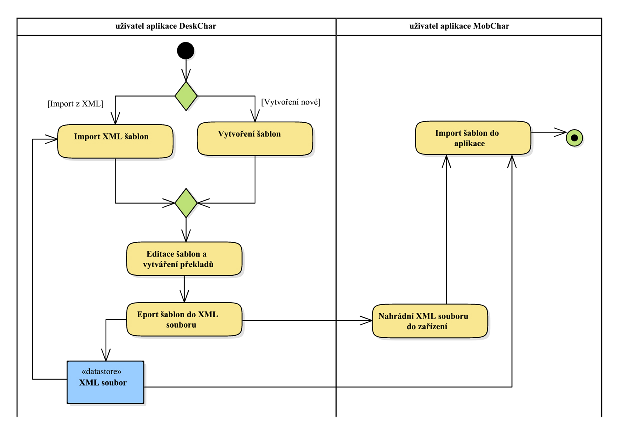
\includegraphics[width=0.8\textwidth]{images/bussiness_sablony}
	\caption[Business proces vytváření šablon]{Model bussines procesů vytváření šablon}\label{fig:bp_sablony}
\end{figure}
Diagram na obrázku \ref{fig:bp_sablony} popisuje základní proces práce se šablonami. Proces popisuje vytvoření šablon a~následné nahrání do mobilní aplikace. Šablony vytvoříme v~programu nebo případně importujeme z~xml souboru vytvořeném buď aplikací nebo například aplikací MobChar. Samozřejmě import a~vytvoření nových šablon můžeme kombinovat. Při tomto procesu nevzniká pouze jedna šablona, ale celý soubor šablon, obvykle jednoho typu. Provedeme veškeré potřebné úpravy a~vytvoříme překlady (pokud jsou nějaké zapotřebí). Danou šablonu následně exportujeme do strukturovaného souboru XML ve~formátu, který podporuje aplikace MobChar. Uživatel mobilní aplikace si vytvořený soubor nahraje do zařízení a~následně provede import do aplikace. Nyní již může s~novou šablonou pracovat.

\subsection{Vytváření dobrodružství}
\begin{figure}\centering
	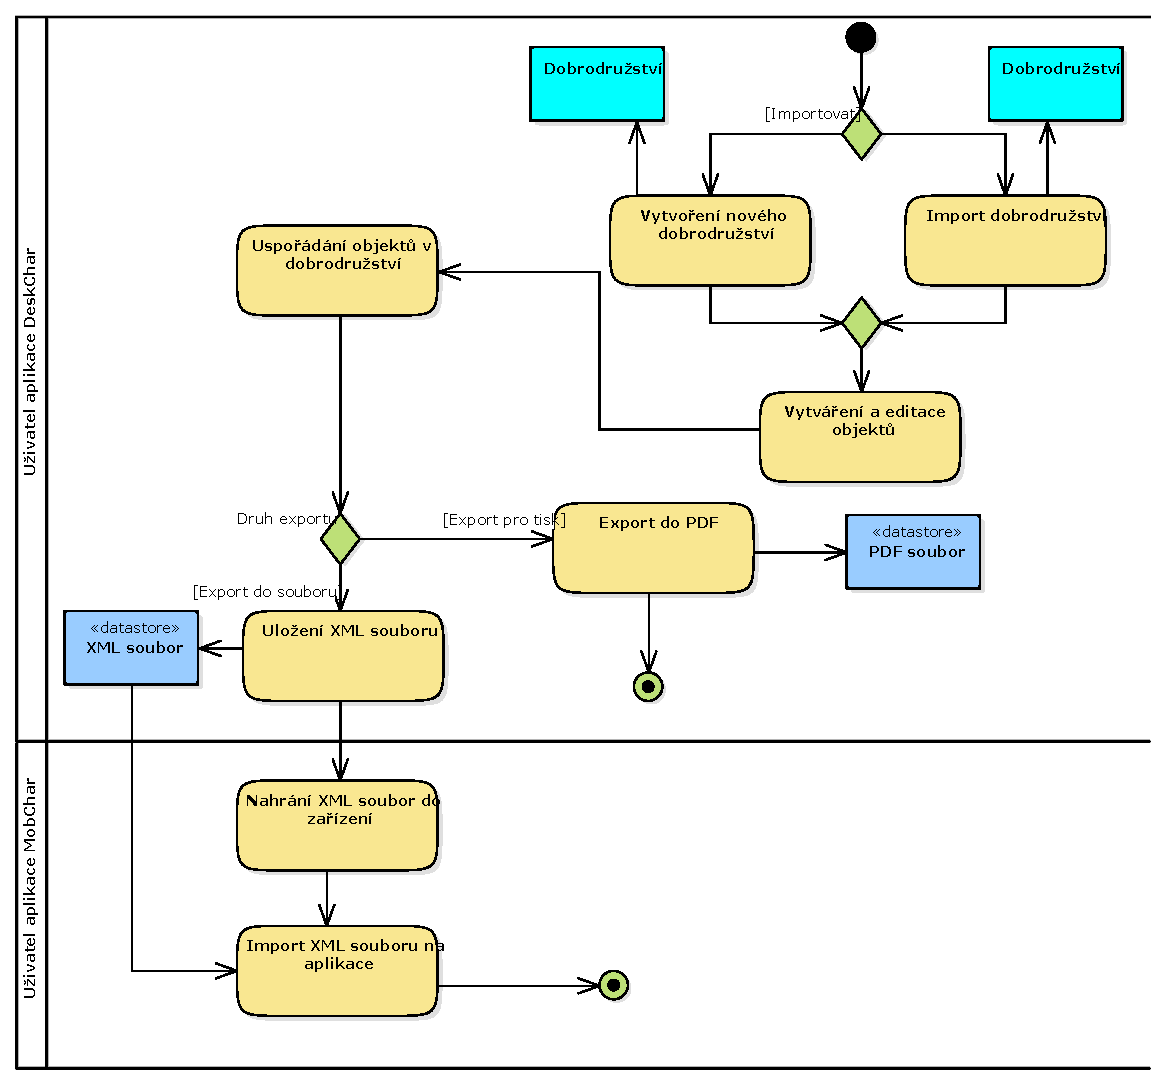
\includegraphics[width=0.8\textwidth]{images/business_dobrodruzstvi}
	\caption[Business proces vytváření dobrodružství]{Model bussines procesů vytváření dobrodružství}\label{fig:bp_dobrodruzsvi}
\end{figure}
Diagram \ref{fig:bp_dobrodruzsvi} popisuje proces, při kterém vzniká nové dobrodružství. Jak už jsem dříve zmiňoval, tak dobrodružství je také šablona. Protože se jedná o hlavní šablonu, která v sobě obsahuje větší počet šablon různých druhů, rozhodl jsem se vytváření dobrodružství popsat více do podrobna. Na začátku procesu vytvoříme nové dobrodružství nebo importujeme již existující a dále budeme upravovat již stávající hodnoty. V bodě \textbf{Vytváření a editace objektů} se jedná o bussines proces popsaný v kapitole \ref{sec:vytvareni_sablon},ve kterém vytvoříme veškeré potřebné objekty, které budou součástí dobrodružství. Do dobrodružství veškeré šablony přidáme a rozřadíme podle potřeby ( podle částí dobrodružství, podle typu šablony atd.). Když máme veškeré úpravy hotové, můžeme výsledné dobrodružství exportovat. Zde si můžeme vybrat zda budeme exportovat dobrodružství pro tisk do formátu PDF nebo pro MobChar ve formátu XML.\\
\textbf{Formát pro tisk:} Vybereme části, které chceme exportovat (nemusíme exportovat celé dobrodružství naráz) a provedeme export. Vytvoří se nám přehledný PDF soubor který následně můžeme vytisknout nebo nahrát do zařízení, které umí pracovat s formátem PDF.\\
\textbf{Formát pro MobChar:} Při exportu do formátu XML se vždy exportuje celé dobrodružství. Nedají se vybrat pouze některé části. Aplikace vytvoří XML soubor. Uživatel následně získaný soubor nahraje do zařízení a importuje ho do aplikace. Takto vytvořené dobrodružství je určené pro MobChar rozšíření pro Pána jeskyně.

%% -*-*-*-*-*-*-*-*-*--* Případy užití *-*-*-*-*-*-*-*-*-*-*-*-*-*-*
	\section{Případy užití}
Případy užití popisují jednotlivé činnosti, které uživatel provádí, při práci s~aplikací. Diagram byl rozdělen na tři hlavní části pro větší přehlednost.
\subsection{Práce se šablonami}
\begin{figure}\centering
	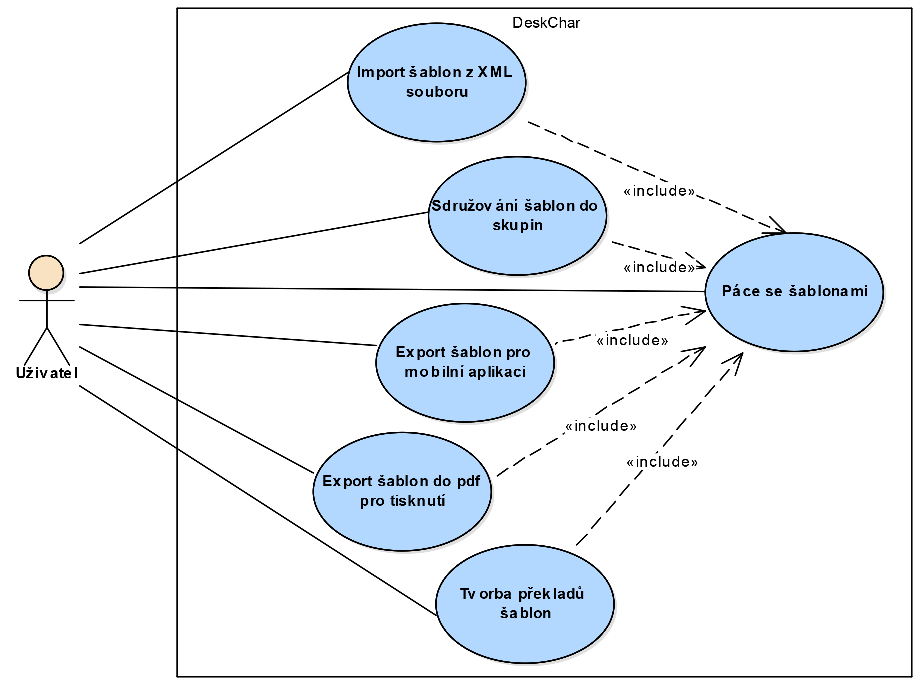
\includegraphics[width=0.8\textwidth]{images/usecase_sablony.pdf}
	\caption[Případy užití pro šablony]{Případy užití pro práci se šablonami}\label{fig:uc_sablony}
\end{figure}

Množina případů užití týkající se práce se šablonami namodelovaná na obrázku \ref{fig:uc_sablony}, se týká veškeré práce se šablonami. Dobrodružství a postavy jsou složené z jednotlivých šablon, které se dají využít i samostatně. Samotné dobrodružství a postavy mají stejný formát jako šablony a navíc můžou obsahovat základní šablony (například postavy můžou mít u sebe zbraně).\\
\\
\textbf{Vytváření a editace šablon:} uživatel si bude moci vytvořit nové šablony nebo editovat stávající. Veškeré parametry, které je možné do šablony zapsat, lze jednoduše upravovat v přehledném formuláři. Uživatel si může vytvořit libovolný počet šablon, které se na základě návazností sdružují do větších celků (dobrodružství, postava).\\
\\
\textbf{Import šablon z XML souboru:} program bude umožňovat import šablon ze strukturovaných XML souborů, které vytváří mobilní aplikace MobChar a také samotný program. Importované šablony se přidají do databáze a lze s nimi následně provádět stejné činnosti jako s nově vytvořenými. Import je možný buď hromadný, který se pokusí ze souboru dostat veškeré dostupné informace a přidat je do aplikace na příslušná místa, nebo lokální import, který ze souboru vytáhne pouze šablony o daném typu.\\
\\
\textbf{Sdružování šablon do skupin:} veškeré šablony půjde rozřazovat do stromové struktury pro větší přehlednost a jednoduší práci s nimi. Pomocí vytváření složek a jednoduchého drag and drop systému bude rozřazování velice jednoduché a intuitivní. Díky rozřazení do složek je následná práce se šablonami velice usnadněná, ať už se jedná o export nebo přiřazování do rodičovských šablon.\\
\\
\textbf{Export šablon:} veškeré vytvořené šablony lze z aplikace exportovat. K dispozici jsou různé druhy exportu. První možnost je export pro mobilní aplikace MobChar. Aplikace vytvoří strukturované XML soubory, které odpovídají formátu, který používá mobilní aplikace MobChar. Další možností exportu je PDF formát, který slouží pro tisknutí šablon do přehledného almanachu, který umožní využít šablony i hráčům, kteří mobilní aplikaci nemají nebo ji nechtějí použít. Poslední možnost exportu, je klasické uložení celého stavu šablon do jednoho xml souboru, který bude využívat stejnou strukturu šablon. \\
\\
\textbf{Tvorba překladů šablon:} ke každé šabloně vytvořené nebo importované do aplikace lze vytvořit neomezený počet překladů. Překlady se vytváří v rámci jedné šablony, pomocí přehledného přepínaní mezi jazyky. Veškeré hodnoty, pro které překlad nemá smysl (číselné hodnoty, povolání, atd.) budou synchronizování napříč všemi jazyky.\\
\\

%% -*-*-*-*-*-*-*-*-*--* Doménový model *-*-*-*-*-*-*-*-*-*-*-*-*-*-*
	\section{Doménový model}
Doménový model má za úkol popsat strukturu tříd v aplikaci a jejich vazby mezi nimi. Pro zaznamenání se využívá UML diagram. Diagram nepopisuje jednotlivé funkce tříd ani proměnné, které slouží k implementaci tříd, ale zachycuje pouze základní strukturu.
\subsection{Stromová struktura}
\begin{figure}\centering
	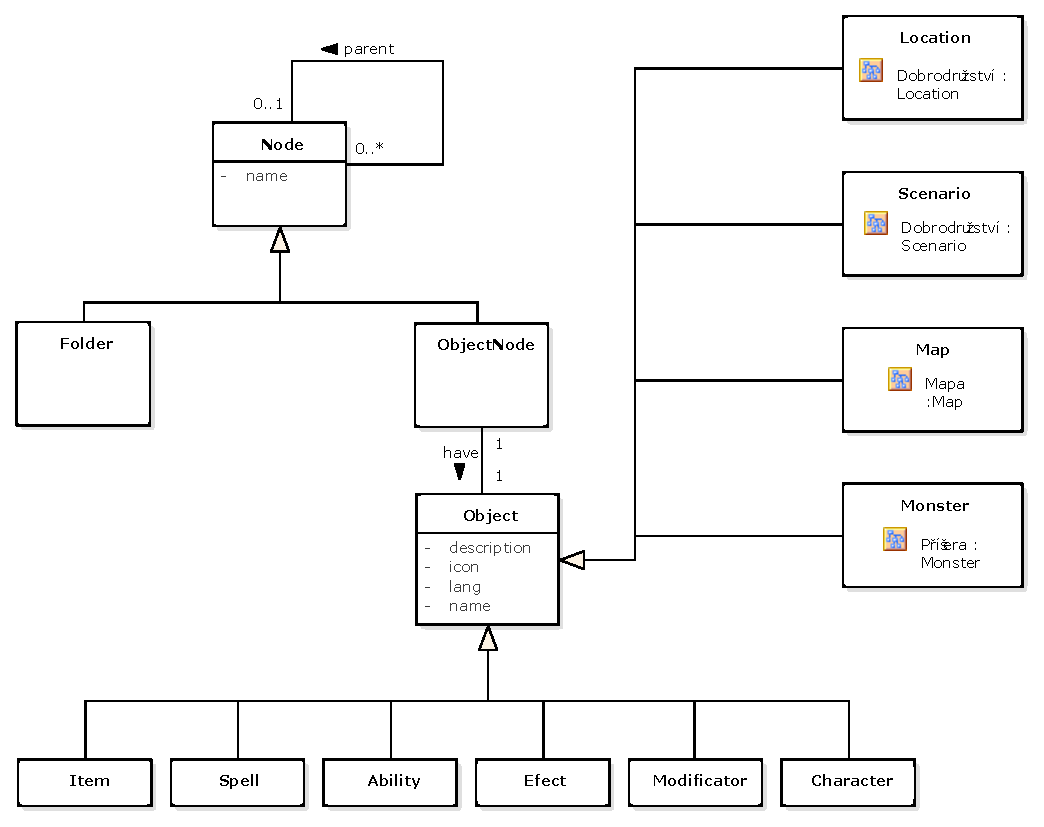
\includegraphics[width=0.8\textwidth]{images/domain_struktura}
	\caption[Analytický doménový model stromové struktury]{Analytický doménový model stromové struktury}\label{fig:dm_stromova_struktura}
\end{figure}
Diagram na obrázku \ref{fig:dm_stromova_struktura} popisuje strukturu objektů, které slouží pro uchování všech objektů (šablon) a jejich rozřazení do stromové struktury. Veškeré šablony využívají tuto stromovou strukturu. Třída Folder (složka) slouží pouze k rozřazování jednotlivých objektů do skupin. Složka má pouze jméno a může obsahovat libovolný počet složek nebo objektů. ObjektNode pak slouží k uchování šablony samotné. Dolní část objektů na obrázku (Item, Spell, atd.) jsou objekty, které jsou totožné s aplikací MobChar a slouží k uchování šablon pro základní aplikaci a využívají se i v aplikaci pro Pána jeskyně. Pokud vás zajímá podrobnější popis těchto objektů, nahlédněte do bakalářské práce týkající se MobCharu \cite{Weberova_2017}. Oproti tomu, objekty na pravé straně diagramu (Map item, Scenario, atd.) jsou objekty, které slouží převážně k vytvoření dobrodružství. Jejich podrobnějšímu popisu se věnuji dále.\\
\\
Veškeré objekty můžou mít potomky. Systém složek slouží pouze pro přehledné uspořádání. Každý objekt má definované objekty, které může mít jako potomky. Tento systém slouží pro ukládání závislostí, například dobrodružství může obsahovat mnoho lokací, příšer, map. Některé objekty, jako například kouzla a schopnosti, žádné potomky mít nesmějí. Veškeré vazby mezi objekty jsou zachyceny pouze ve stromové struktuře, aby bylo zabráněno duplikování informací.
\subsection{Dobrodružství}
\begin{figure}\centering
	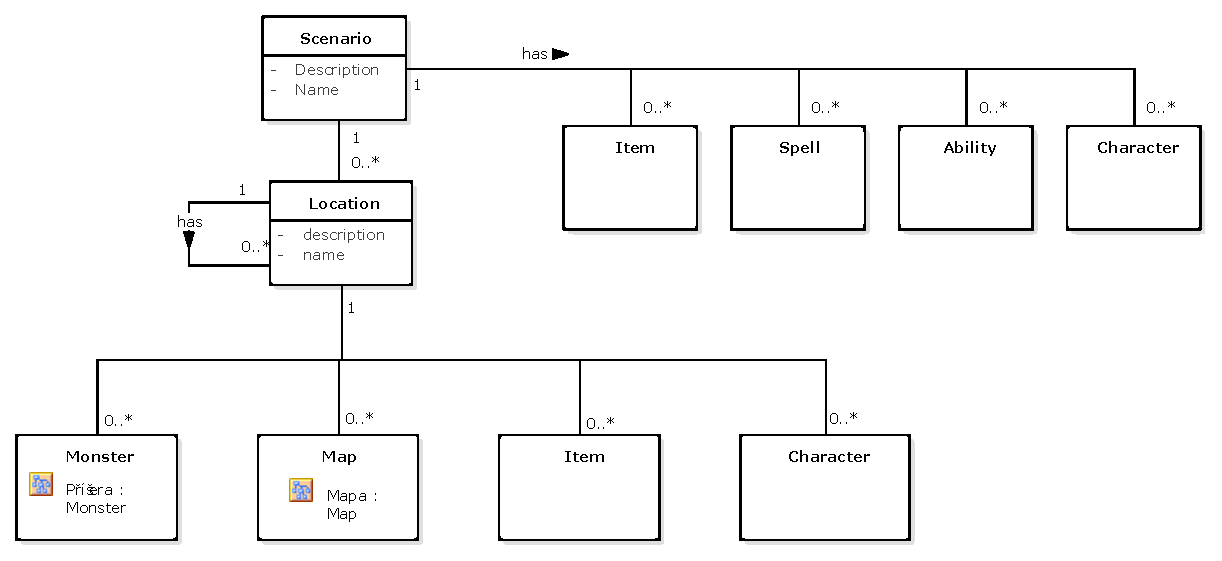
\includegraphics[width=0.8\textwidth]{images/domain_scenario}
	\caption[Analytický doménový model dobrodružství]{Analytický doménový model dobrodružství}\label{fig:dm_scenario}
\end{figure}
Diagram na obrázku \ref{fig:dm_scenario} popisuje strukturu pro ukládání a práci s dobrodružstvím. Hlavní třída \textit{scenario} je rozdělená do jednotlivých lokací. Pro celé dobrodružství jsou však společné předměty, kouzla, schopnosti a postavy. Předměty, kouzla a schopnosti jsou pro P	ána jeskyně, který je nadále poskytuje hráčům, například pokud se hráč má možnost naučit nové kouzlo, nebo získal důležitý předmět pro dobrodružství (elixír, mapa, atd.). Třída \textit{Character} zde zastupuje postavy hráčů, kteří dané dobrodružství hrají. Jedná se o stejné třídy jako v původní aplikaci MobChar. Pro přesnější popis těchto tříd, nahlédněte do bakalářské práce aplikace MobChar\cite{Weberova_2017}.\\
\\
Celé dobrodružství je členěné do lokací, které se navíc můžou do sebe zanořovat (lokace může mít pod sebou další lokace). Lokace obsahují příšery, mapy, předměty a postavy. Příšery mají velice podobnou strukturu jako postavy, můžou se naučit schopnosti a kouzla a vlastnit předměty, mají však odlišné atributy, proto jsou od postav odděleny. Jednotlivé mapy mají složitější strukturu, která je popsána níže. Předměty zde znamenají předměty důležité pro tuto lokaci (klíče, věci v bednách a další). Poslední částí jsou postavy, které zde znázorňují postavy, za které nehrají hráči, ale samotný PJ. Jsou to důležité postavy pro dobrodružství, které se nacházejí v dané lokaci. Objekt je stejný jako klasické postavy, ale význam je trochu odlišný.




	\section{Návrh řešení architektury}
\begin{figure}\centering
	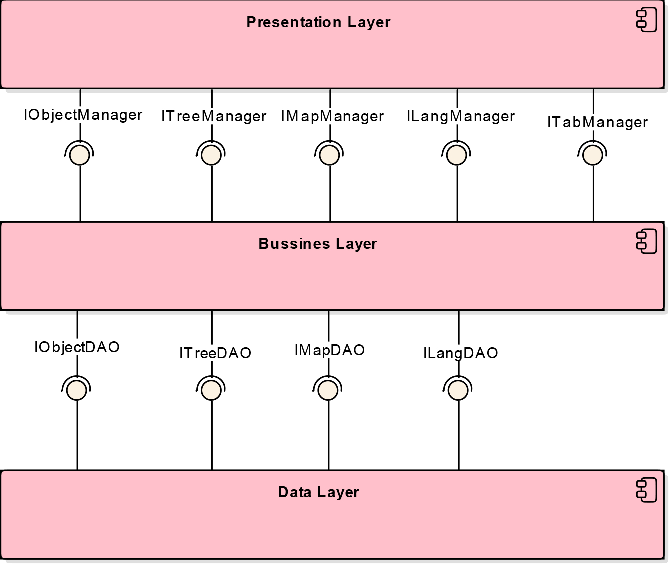
\includegraphics[width=0.8\textwidth]{images/architektura}
	\caption[Model architektury]{Model architektury}\label{fig:architektura}
\end{figure}
Model architektury popisuje formální popis systému, případně jeho detailní plán na úrovni komponent vedoucí k jeho implementaci. Hlavním účelem modelu architektury je popsání hlavních komponent programu a popisu způsobu komunikace mezi nimi.\\
\\
Zvolil jsem třívrstvou architekturu z důvodu dobré přehlednosti a jednoduchém nahrazení jedné z části, bez zásahu do ostatních vrstev. Veškeré vrstvy mezi sebou komunikují na základě definovaného rozhraní.\\
\subsection{Vrstvy}
\textbf{Prezentační vrstva} zobrazuje informace pro uživatele. Jedná se o grafickou část celé aplikace. Kontroluje zadané vstupy, nijak však získaná data nezpracovává.\\
\textbf{Business vrstva} je základní logická část aplikace. Leží zde jádro aplikace, její logika a funkce pro zpracování dat.\\
\textbf{Datová vrstva} je vrstva, která se stará o práci s daty. Zajišťuje komunikaci s databází a práci s XML soubory. Jejím základním úkolem je získat data z databáze nebo XML a převést je na objekty a také objekty vytvořené v aplikaci uložit do databáze nebo případně do XML souborů. \\
\subsection{Rozhraní}
Mezi vrstvami jsou definovaná rozhraní, která je nutné dodržet. Rozhraní začínají velkým písmenem I, konkrétní implementace daného rozhraní obvykle má stejný název, pouze bez počátečního písmena I.\\
\\
Pro datovou vrstvu se používají takzvané \clqq data access objects\crqq (DAO). Jedná se o třídy, které zajišťují přístup k datům například z databáze a naopak i data ukládají. Pro business vrstvu se využívají takzvané \clqq managery\crqq .
\subsubsection*{DAO třídy}
\noindent\textbf{IObjectDAO} je skupina několika DAO tříd, které se starají o přístup k datům z databáze a z XML. Na diagramu \ref{fig:architektura} je zobrazen pouze zástupný IObjectDAO, který v implementaci neexistuje a je nahrazen jednotlivými DAO rozhraními (ISpellDAO, IEffectDAO atd.).\\
\\
\textbf{ITreeDAO} se stará o~veškeré ukládání stromové struktury do databáze. \\
\\
\textbf{IMapDAO} se stará o ukládání veškerých dat, která se týkají map. Rozhraní je společné pro všechny druhy map (grafické, jednoduché, obrázkové)\\
\\
\textbf{ILangDAO} se stará o ukládání jazyků, které jsou v aplikaci použity. Nejedná se o překlady prezentační vrstvy, ale o jazyky vytvořené pro překlady šablon. Rozhraní se nestará o ukládání samotných překladů, pouze o jejich jazyky.

\subsubsection*{Manager třídy}
\textbf{IObjectManager} navazuje na IObjectDAO. Jedná se opět o skupinu tříd pro veškeré základní objekty (ISpellManager, IAbilityManager, atd.). Rozhraní definuje, jak přijímá data z prezentační vrstvy. Základní funkcionalita spočívá ve zpracování dat z prezentační vrstvy a vytvoření kompletního objektu, se kterým se dále pracuje nebo se pošle na datovou vrstvu pro uložení.\\
\\
\noindent\textbf{ITreeManager} se stará u připravení stromové struktury pro zobrazení. Vytváří z objektů stromovou strukturu a přidává do struktury metadata, které slouží pro zobrazení a práci na prezentační vrstvě.\\
\\
\textbf{IMapManager} se stará o zpracování dat ohledně mapy. Převádí zobrazenou mapu pro uživatele na formu, ve které se dá snadno uložit do databáze. Propojuje veškeré šablony s mapou.\\
\\
\textbf{ILangManager} se stará o zpracování dat z prezentační vrstvy ohledně jazyků.\\
\\
\textbf{ITabManager} se stará o vytváření překladových záložek pro prezentační vrstvu. Toto rozhraní nemá DAO rozhraní, protože veškeré informace které potřebuje, získá přímo z konkrétních IObjectDAO tříd. Jejím hlavním úkolem je zpracování všech překladů jedné šablony a připravení objektů pro uložení.\\





\chapter{Návrh}
	\section{Model databáze}
	\begin{figure}\centering
	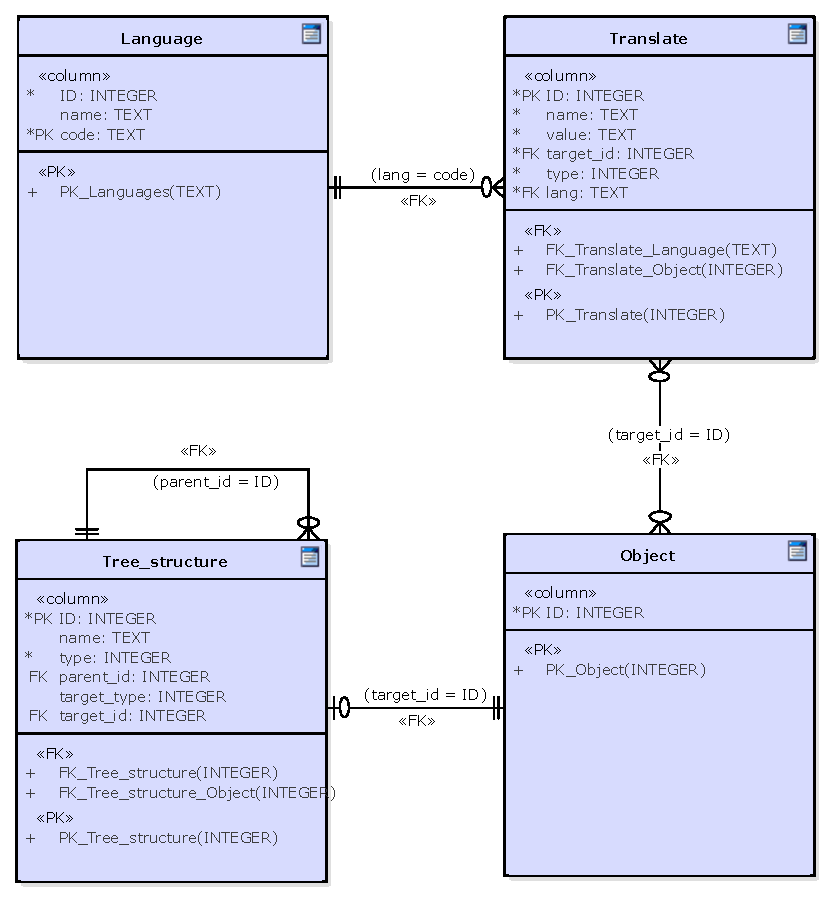
\includegraphics[width=0.8\textwidth]{images/basic_database}
	\caption[Základní model databáze]{Základní model databáze}\label{fig:db_basic}
	\end{figure}
	Pro realizaci aplikace DeskChar jsem vybral databázi \textit{SQLite}, která je jednoduchá a nepotřebuje žádný složitý externí software pro běh. Na druhou stranu zvládá veškeré potřebné operace, jako jsou cizí klíče a kaskádové mazání záznamů. Pro vytváření a práci se stromovou strukturou je kaskádové mazání nedocenitelný pomocník. \\
\\
Diagram na obrázku \ref{fig:db_basic} je zjednodušený pro větší přehlednost. Na diagramu je zachycena základní struktura a princip závislostí v~databázi. Kompletní model databáze se nachází v~příloze.\\
\\
Z důvodu vícejazyčnosti šablon, bylo zapotřebí navrhnout strukturu databáze, která dokáže uložit neomezený počet jazykových překladů. Na obrázku \ref{fig:db_basic} můžeme vidět základní strukturu databáze. Údaj o jazyku, ve kterém je daný překlad vytvořen, je uložen v tabulce \textit{Languages}, který je navázán na tabulku \textit{Translate} cizím klíčem code. Primárním klíče každého jazyka je textový kód, který je unikátní. V tabulce \textit{Translate} pak nalezneme veškeré textové řetězce, které se nacházejí v objektech. Jeden záznam tabulky \textit{Translate} je přiřazen ke konkrétnímu objektu pomocí dvojice klíčů target\_type, který určuje o jaký objekt (tabulku v databázi) se jedná, a \textit{target\_id}, který určuje konkrétní záznam v tabulce (ukazuje na primární atributů \textit{ID} v tabulce). Informace o překladu jsou uloženy ve dvojici atributů \textit{name} a \textit{value}, které slouží jako slovník, jejich jazyk určuje atribut \textit{lang}. Takto zvolený návrh databáze umožňuje neomezený počet jazyků a jednoduchou rozšiřitelnost.\\
\\
Druhá část diagramu se týká stromové struktury, která se používá pro všechny objekty v aplikaci. Tabulka \textit{Tree\_structure} slouží pro zaznamenávání stromové struktury pro veškeré objekty. Do tabulky se ukládají dva druhy uzlů, složky a objekty. Atribut type určuje, o který druh uzlu se jedná. Pomocí cizího klíče \textit{parent\_id}, vzniká stromová struktura. Zde se využívá kaskádové mazání - pokud se smaže záznam, který má pod sebou navázané další záznamy pomocí cizího klíče, smažou se tyto záznamy také automaticky v databázi. Tento princip udržuje tabulku konzistentní a nevznikají žádné záznamy, které se již nepoužívají. Každý uzel, který je typu object, ukazuje pomocí dvojice klíčů \textit{target\_type}, který určuje tabulku v databázi, a \textit{target\_id} na záznam v ostatních tabulkách. V diagramu je to naznačené zjednodušeně, kde tabulka \textit{Object} zastupuje tabulky všech objektů (Spell, Item, atd.). \\
\\
Poslední problém návrhu databáze se skrýval v návrhu ukládání vazeb mezi jednotlivými objekty. V úvahu připadali dvě možnosti. První možnost byla zachytit veškeré vazby mezi objekty pomocí tabulek relations, které by obsahovaly pouze dvojici klíčů z obou tabulek. Toto řešení by bylo rychlé a jednoduché na používání, bohužel se u některých vazeb nedalo použít samotné. Například u dobrodružství se podřazené objekty můžou sdružovat dále do složek, čehož by se pouze pomocí těchto vazeb nedalo docílit. Musela se zde navíc využít stromová struktura použitá pro všechny šablony a jejich základní rozřazení, čímž by vznikaly duplicitní data. Duplicitní data sebou nesou dva základní problémy. První z nich je samozřejmě větší množství dat, které je potřebné uložit. V tomto případě by se však nejednalo o drastický nárůst, který by dělal problém. Druhý a závažnější problém se týká aktuálnosti dat. Bylo by zapotřebí udržovat veškeré údaje aktuální a stejné, což by mělo velké nároky na složitost ukládání a zpomalovalo by to některé operace, které je zapotřebí, aby aplikace prováděla okamžitě (například drag and drop rozřazování). Z těchto důvodů jsem se rozhodl zvolit druhou možnost, kde veškeré vazby mezi objekty jsou uloženy pouze ve stromové struktuře popsané výše. Problém bude vznikat při operacích exportu, kde bude vazbu mezi objekty dohledávat ze stromové struktury. Tyto operace se však neprovádí tak často a není zde velký důraz na okamžitou odezvu. 

	\section{Model XML souborů}
S~doménovým modelem úzce souvisí návrh struktury xml souborů. Struktura těchto souborů je velmi důležitá. Na základě této definované struktury bude probíhat komunikace s~mobilní aplikací MobChar. Formát základních šablon předmětů, kouzel, schopností, efektů a~postav, byl převzat z~původní aplikace MobChar pro hráče, aby byla zachována konzistence mezi aplikacemi. Dále se zaměřuji pouze na nové části, což jsou příšery a dobrodružství. Pokud vás zajímá struktura základních šablon, nahlédněte do bakalářky týkající se aplikace MobChar\cite{Weberova_2017} nebo do přiložené kompletní dokumentace.\\
\\
Strukturu XML jsem namodeloval diagramem, který se normálně využívá pro modelování tříd. Pro tento případ vypovídající hodnota diagramu je dostačující a jasně zadefinovává strukturu xml. Entity v diagramu které jsou znázorněné žlutou barvou znázorňují již konkrétní XML tag, který uvnitř obsahuje pouze hodnotu a žádné další vnořené tagy. Oproti tomu bílé entity znázorňují pouze obalující tag, který uvnitř obsahuje strukturu další tagů. Každá entita v diagramu znázorňuje jeden tag ve výsledném XML dokumentu. Parcialita a kardinalita v diagramu znázorňuje povinnost případně množství tagů, které se na daném místě v XML souboru můžou objevit. Kořenový tag je vždy označen textem  \clqq ROOT\crqq .

\subsection{Dobrodružství}
\begin{figure}\centering
	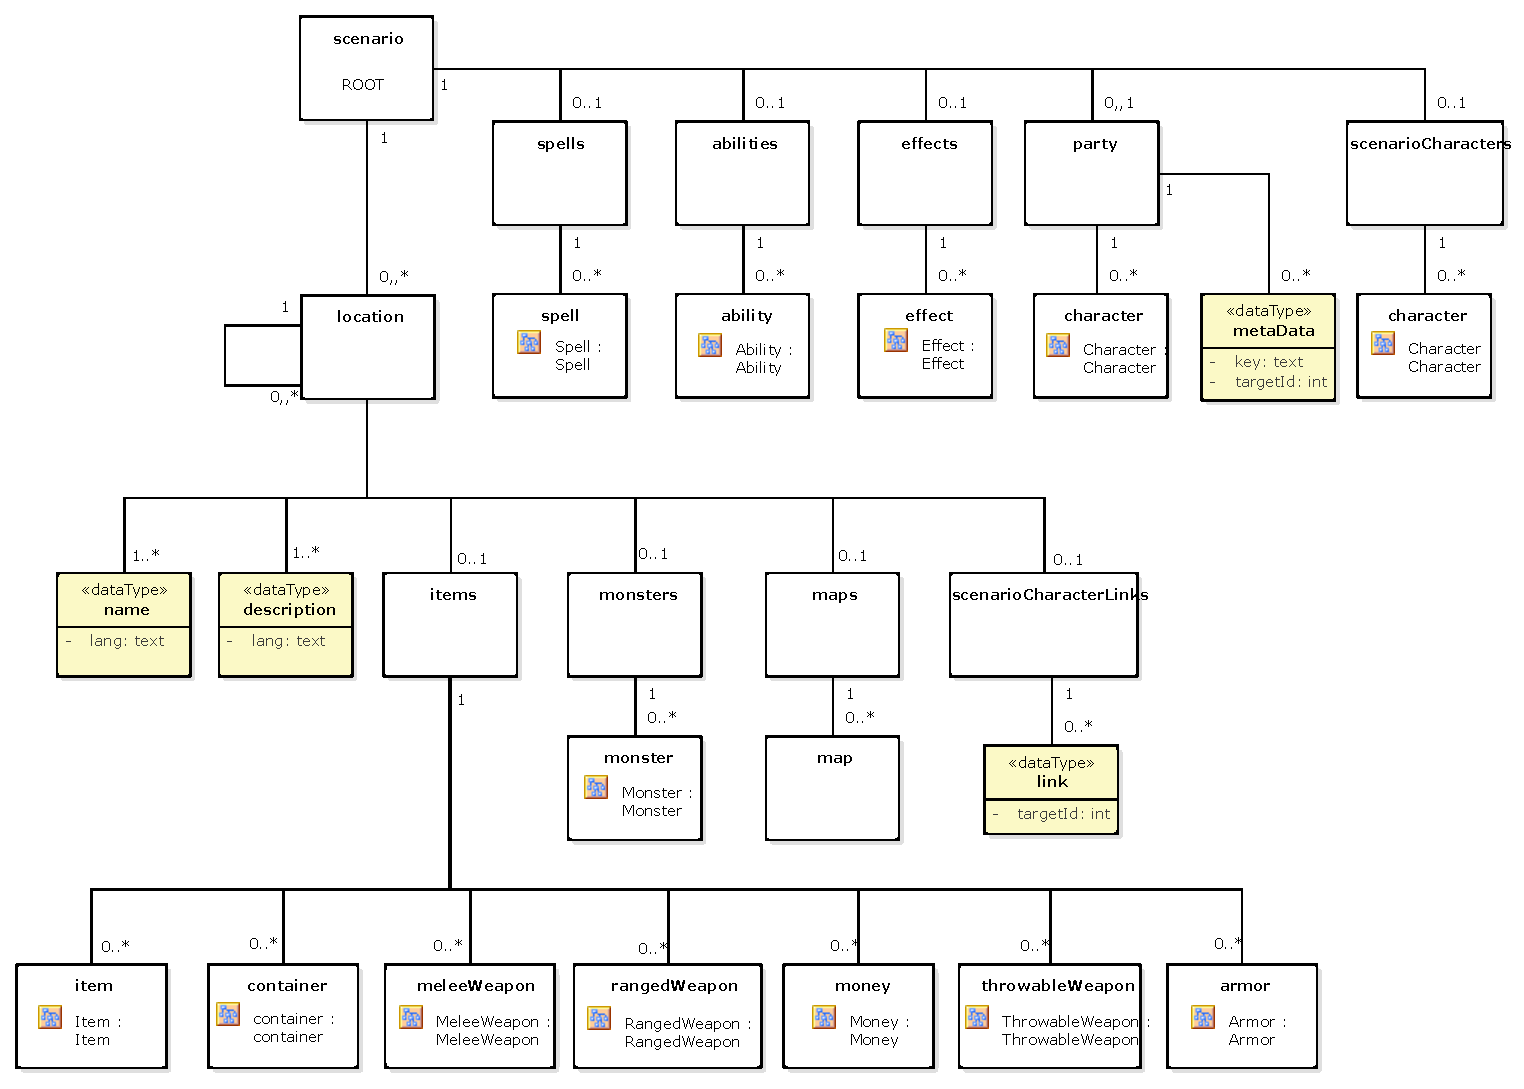
\includegraphics[width=0.8\textwidth]{images/scenarioXML}
	\caption[Model XML souhoru dobrodružství]{Model XML souhoru dobrodružství}\label{fig:xml_scenario}
\end{figure}
Struktura xml souboru pro dobrodružství je velice podobná doménovému modelu dobrodružství, jak můžeme vidět na obrázku \ref{fig:xml_scenario}. První z odlišností si můžeme všimnout tagu \clqq metaData\crqq . Tato data využívá pouze mobilní aplikace MobChar a slouží pro ukládání metadat ohledně připojených uživatelů. Tyto údaje v aplikaci nejdou nijak upravovat a pouze se ukládají pro udržení informace při importu a exportu. \\
Další odlišnost se nachází u \clqq scenarioCharacter\crqq . Z důvodu zachování historie cizích postav napříč lokacemi, se v lokacích nachází pouze link na postavu, která je definovaná pro celé dobrodružství. Jedná se o seznam tagů se jménem \textit{link}, který má obsah pouze identifikátor konkrétní cizí postavy. \\
Poslední významný rozdíl se týká rozdělení předmětů. Předměty jsou rozděleny na 7 kategorií. V aplikaci je dělení stejné, nicméně zde každý předmět má vlastní kořenový tag, čímž je jasně definován. Pokud vás zajímá přesný popis jednotlivých předmětů, můžete nahlédnout do přiložené dokumentace. \\

\subsection{Příšery}
\begin{figure}\centering
	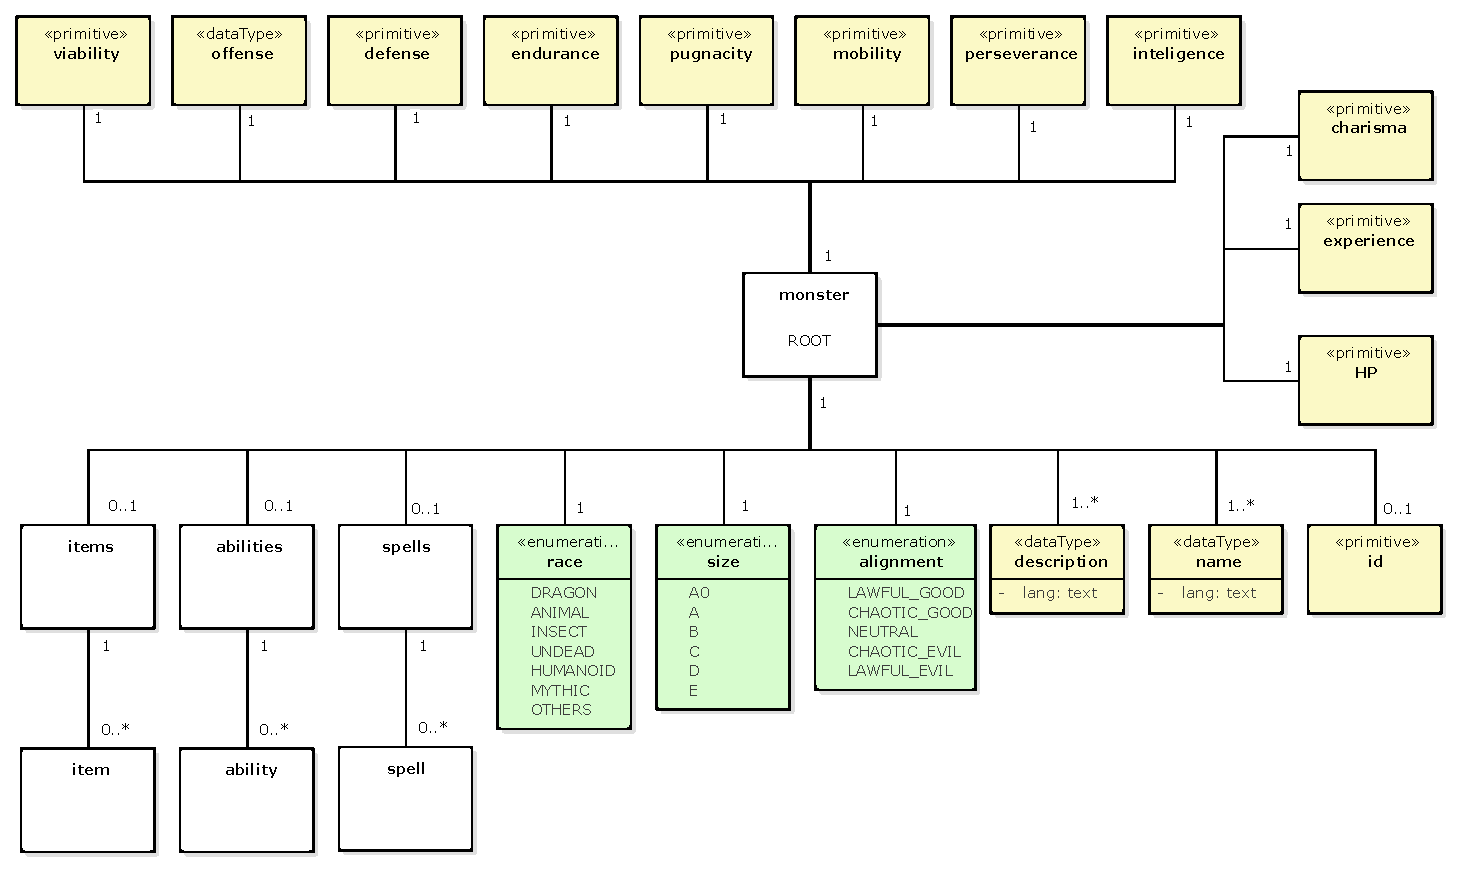
\includegraphics[width=0.8\textwidth]{images/monsterXML}
	\caption[Model XML souhoru příšery]{Model XML souhoru příšery}\label{fig:xml_monster}
\end{figure}
Druhý nově zadefinovaný formát xml souborů se týká příšer. Příšery jsou samozřejmě součástí dobrodružství, jak jste mohli vidět na obrázku \ref{fig:xml_scenario}. Na obrázku \ref{fig:xml_monster} můžeme vidět detailní strukturu souboru. Struktura je podobná postavám, také obsahuje seznam předmětů, schopností a kouzel. Také obsahuje tag race, který určuje rasu příšery, ale jedná se o odlišné rasy než pro postavy. Pro určení rasy příšer jsme hledali kompromis, mezi dostatečnou vypovídající hodnotou a konzistencí oproti velkému množství ras, které by se velice rychle stalo nepřehledné. Uživatel si samozřejmě může příšery rozřadit podle libosti na základě stromové struktury nebo případně v popisku příšery. Proto jsme se rozhodli rasy příšer omezit pouze na základních sedm, které můžete vidět na obrázku. Hlavní důvod rozdělení příšer od klasických postav byl v rozdílných atributech. Pro počítání výsledku soubojů se používají jiné atributy než u postav. 



	\section{Model komunikace}
	\begin{figure}\centering
	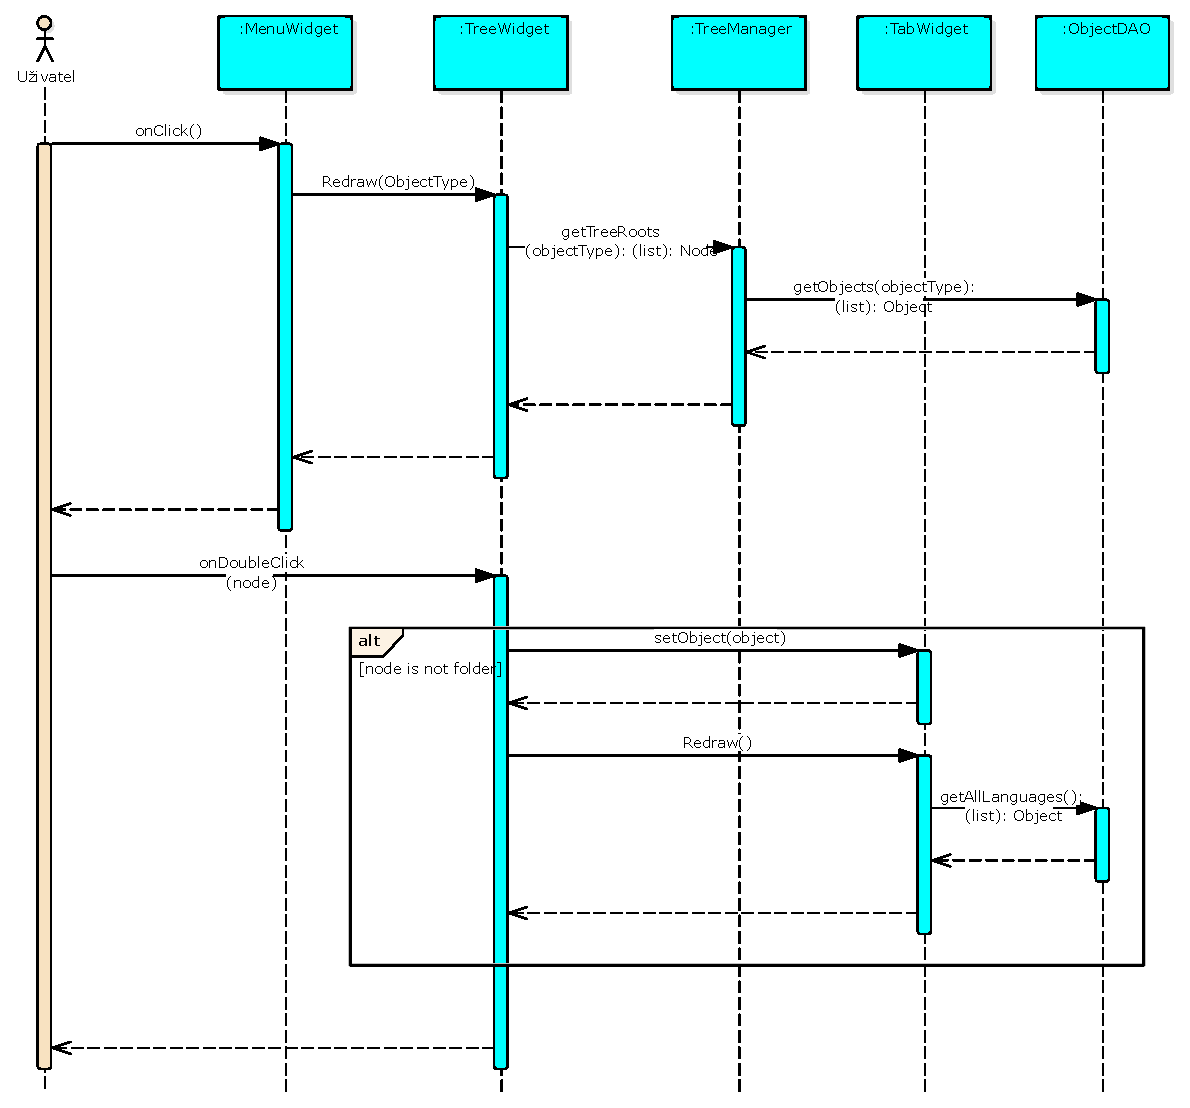
\includegraphics[width=0.8\textwidth]{images/comunication_main}
	\caption[Model komunikace pro hlavní obrazovku]{Model komunikace pro hlavní obrazovku}\label{fig:comunication_main}
	\end{figure}
Nejčastější operaci prezentační vrstvy je práce se stromovou strukturou a vytváření překladů. Pro znázornění komunikace mezi vrstvami jsem vytvořil sekvenční diagram, který znázorňuje komunikaci mezi jednotlivými třídami prezentační vrstvy. Na diagramu \ref{fig:comunication_main} můžeme vidět základní dvě činnosti. Vybrání konkrétního typu šablon , které zobrazí stromovou strukturu a zobrazení hlavního widgetu pro vytváření šablon po vybrání konkrétní položky ve stromové struktuře.\\
\\
Uživatel v menu klikne na požadovaný druh šablon. Tím se zavolá funkce \textit{Redraw}, která má na starosti vykreslení stromové struktury ve widgetu. Potřebná data získá z \textit{TreeManageru} po zavolání funkce \textit{getTreeRoots}, která má na starosti, vytvoření kompletního stromu uzlů, přičemž vrací seznam kořenových uzlů. \textit{TreeWidget} z tohoto listu pomocí rekurze vykreslí celý strom. \textit{TreeManager} získává data z konkrétní DAO třídy (v diagramu zjednodušena jako \textit{ObjectDAO}). Objekty navěšené na uzly stromu můžou být různé, takže třída \textit{TreeManager} volá více DAO tříd.\\
\\
Druhá část diagramu se týká vykreslení hlavní části obrazovky, kde se vytváří samotné šablony a jejich překlady. Uživatel v \textit{TreeWidgetu} dvakrát klikne na nějaký uzel. Pokud se jedná o složku, funkce zavolá pouze rodičovskou funkci \textit{TreeWidgetu}, což má za následek rozbalení obsahu složky. Pokud se jedná o objekt, zavolá se nad třídou \textit{TabWidget} funkce \textit{setObject} s parametrem object. Hned poté se zavolá funkce, která vykreslí všechna data. Data získá na základě nastaveného objektu, který si pamatuje vlastní DAO třídu. Třída vrátí seznam objektů, přičemž se jedná o jednu šablonu, ale ve všech jazycích, ve kterých byla vytvořena. \textit{TabWidget} následně pro každý jazyk vykreslí jednu záložku, kde se dají hodnoty šablony upravovat nebo případně vytvořit nový překlad pro nový jazyk.
	
	\section{Model nasazení}
	\begin{figure}\centering
	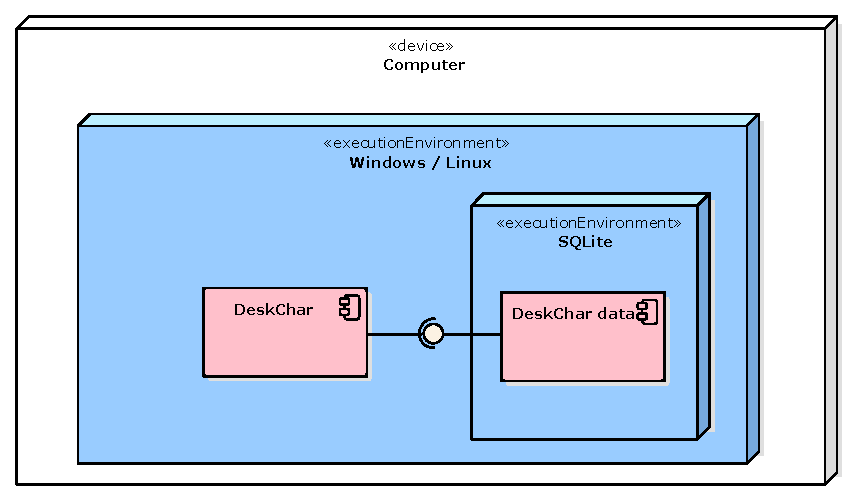
\includegraphics[width=0.8\textwidth]{images/model_nasazeni}
	\caption[Model nasazení]{Model nasazení}\label{fig:model_nasazeni}
	\end{figure}
Diagram nasazení zobrazuje způsob rozdělení systému na samostatné části a komunikační vazby mezi nimi, čímž definuje architekturu systému. Nalezneme zde veškeré komponenty systému a všechny potřebné části pro běh naší aplikace.\\
\\
Na diagramu \ref{fig:model_nasazeni} můžeme vidět, že software je určený pro počítače a funkční pod operačními systémy Windows a Linux (verze operačního systému jsou uvedeny v sekci nefunkční požadavky \ref{sec:funkcni_pozadavky}). Aplikace je napsaná v jazyce Python a zabalená do spustitelného balíčku, který nevyžaduje žádné speciální požadavky na systém. Veškeré potřebné knihovny a prostředí má uložené v balíčku. Databáze SQLite běží v rámci tohoto balíčku také a nepotřebuje žádné dodatečné prostředí.

\chapter{Realizace}
\section{Použitý programovací jazyk}

\section{Využité knihovny}
\subsection{Knihovna pro práci s XML}
Velká část programu se týká práce s XML šablonami. Bylo zapotřebí vybrat vhodnou knihovnu, která by veškerou práci co nejvíce usnadnila. Hledal jsem knihovnu, která by dokázala namapovat třídu a její atributy přímo na XML šablony. Bohužel taková knihovna pro Python neexistuje. Proto jsem využil knihovnu lxml\cite{lxml}, která umí základní parsování XML souborů a napsal jsem pro ní rozšíření, které umožňuje mapovat objekty přímo na strukturu XML souboru. V ukázce kódu \ref{code:XMLTemplates} můžeme vidět namapování objektů \textit{Effect} a \textit{Modifier} a jejich vzájemné provázání. \\
Rozšíření obsahuje tři základní třídy, \textit{XElement}, \textit{XAttribElement} a \textit{XInstance}. Každá z těchto tříd reprezentuje jiný typ atributu v objektu. Třída \textit{XElement} reprezentuje základní atribut, který nemá překlady. Jako parametr, kromě jména tagu, přijímá volitelný atribut enum, kterým se dá nastavit, že hodnota se má mapovat na konkrétním enum.\\
Třída XAttribElement reprezentuje tagy, které mohou navíc obsahovat atribute. Nejčastěji se to využívá u atributů, které jsou vícejazyčné. Atributem lang se zde nastavuje jazyk překladu.\\
Poslední třída XInstance reprezentuje vazbu na další mapovací třídu. Jako parametr komě jména, přijímá instanci cílové mapovací třídy.\\
\\
Třída \textit{XMLTemplate}, ze které všechny mapovací třídy dědí, obsahuje dvě základní funkce, \textit{import\_xml} a \textit{create\_xml}. Funkce \textit{import\_xml} načte XML soubor a vrátí seznam objektů, které se dále načítají do databáze. O proti tomu třída \textit{create\_xml} přijímá seznam objektů, ze kterých vytvoří strukturovaný XML soubor.


%\begin{lstlisting}[float,language=Python, label=python_xml, caption=Mapování objektů na xml strukturu]
\begin{listing}[htbp]
\caption{\label{code:XMLTemplates}Mapování objektů na XML strukturu}
%\inputminted{python}[linenos]{resources/XMLTemplate.py}
\begin{minted}[]{python}
class XMLModifier(XMLTemplate):
    ROOT_NAME = 'modifier'
    OBJECT_TYPE = ObjectType.MODIFIER%


    def __init__(self):
        self.id = XElement('id')
        self.valueType = XElement('valueType', ModifierValueTypes)
        self.value = XElement('value')
        self.targetType = XElement('targetType')
        self.valueTargetAttribute = XElement('valueTargetAttribute')


class XMLEffect(XMLTemplate):
    ROOT_NAME = 'effect'
    OBJECT_TYPE = ObjectType.EFFECT


    def __init__(self):
        self.id = XElement('id')
        self.name = XAttribElement('name', 'lang')
        self.description = XAttribElement('description', 'lang')
        self.targetType = XElement('targetType')
        self.modifiers = XInstance('modifiers', XMLModifier)
\end{minted}
\end{listing}

\subsection{Grafická knihovna}
Pro Python existuje velké množství grafických knihoven. Některé jsou zaměřené na mobilní aplikace, některé hlavně pro webové rozhraní. Vybrat mezi takovým množstvím knihoven není lehké. Mezi nejznámější patří knihovny Kivy, PyGame, TkInter a PyQt. Knihoven existují desítky další, ale v této bakalářce se věnuji pouze nejzajímavějším z nich.\\
Knihovna kivy je převážně zaměřené na dotykové displeje. Výsledný vzhled a veškeré widgety jsou pro to přizpůsobené a ovládání pomocí myši a klávesnice není tak intuitivní jako u ostatních knihoven.\\
Dalším důležitým kritériem pro výběr knihovny byla aktuálnost a vydávání nových aktualizací. Pro knihovna TkInter již dlouho nevychází nové aktualizace. Knihovna je velice jednoduchá a intuitivní, bohužel již několik let není aktuální. \\
Knihovna PyGame, jak již napovídá její název, se specializuje převážně na tvorbu počítačových her. Má rozsáhlé možnosti animací a herních prvků, které jsou důležité převážně ve hrách. Knihovna neumí vytvářet přehledné grafické rozhraní aplikace, proto jsem ji ze seznamu také vyřadil.\\
Poslední z čtveřice knihoven je PyQt. Knihovna se zaměřuje na tvorbu přehledných grafických rozhraní pro programy, což je přesně to co je zapotřebí. Navíc má velice moderní a přehledný vzhled, což bylo jedno z hlavních kritérii pří výběru. Aktualizace k této knihovně jsou vydávány pravidelně a nejnovější verze PyQt5 je určena pro Python 3. Proto jsem se rozhodl zvolit tuto knihovnu pro můj program.
\subsection{Knihovna pro tvorbu PDF almanachů}

\begin{conclusion}
	%sem napište závěr Vaší práce
\end{conclusion}

\bibliographystyle{resources/csn690}
\bibliography{resources/mybibliographyfile}

\appendix

\chapter{Seznam použitých zkratek}
% \printglossaries
\begin{description}
	\item[HnH] Hra na hrdiny
	\item[DrD] Dračí doupě
	\item[RPG] Role-playing game
	\item[PJ] Pán jeskyně
	\item[DAO] Data access object
	\item[MobChar] Mobile character
	\item[DeskChar] Desktop character
	\item[enum] Enumeration
\end{description}

 

\chapter{Obsah přiloženého CD/USB}

%upravte podle skutecnosti

\begin{figure}
	\dirtree{%
		.1 readme.txt\DTcomment{stručný popis obsahu CD}.
		.1 exe\DTcomment{adresář se spustitelnou formou implementace}.
		.1 src.
		.2 impl\DTcomment{zdrojové kódy implementace}.
		.2 thesis\DTcomment{zdrojová forma práce ve formátu \LaTeX{}}.
		.1 text\DTcomment{text práce}.
		.2 thesis.pdf\DTcomment{text práce ve formátu PDF}.
		.2 thesis.ps\DTcomment{text práce ve formátu PS}.
	}
\end{figure}

\end{document}
